\documentclass[conference]{IEEEtran}

% ── Packages ──
\usepackage[utf8]{inputenc}
\usepackage[T1]{fontenc}
\usepackage{cite}
\usepackage{amsmath,amssymb}
\usepackage{booktabs}
\usepackage{multirow}
\usepackage{graphicx}
\usepackage{pgfplots}
\usepackage{pgfplotstable}
\pgfplotsset{compat=1.18}
\usepackage{xcolor}
\usepackage{caption}
\usepackage[hidelinks]{hyperref}
\usepackage{algorithm}
\usepackage{algpseudocode}
\usepackage{array}
\usepackage{url}
\captionsetup{font=small,labelfont=bf}

\definecolor{lstm}{HTML}{4C72B0}
\definecolor{deeponet}{HTML}{DD8452}
\definecolor{patchtst}{HTML}{55A868}
\definecolor{tirex}{HTML}{C44E52}
\definecolor{randomforest}{HTML}{228B22}
\definecolor{tcn}{HTML}{FF6347}
\definecolor{fkmad}{HTML}{9467BD}
\definecolor{mambasl}{HTML}{8C564B}
\definecolor{convtimenet}{HTML}{17BECF}

\begin{document}

\title{Deep Learning Architectures for Offshore Production Monitoring: A Comparative Benchmark on Fault Detection and Gas Forecasting}

\author{
\IEEEauthorblockN{Samarone Lima Santos J\'{u}nior}
\IEEEauthorblockA{Laborat\'{o}rio de Processamento de Sinais (LPS)\\
Universidade Federal do Rio de Janeiro\\
Rio de Janeiro, Brazil\\
\textit{MSc Thesis --- Preliminary Results}}
}

\maketitle

\section*{Validity Notice (May 2026)}
This IEEE-style draft is retained as historical narrative only. Several result
claims below predate the final post-fix dissertation evidence pack. Current
claims must be taken from \texttt{reports/dissertation\_claim\_ledger\_2026-05.md}
and \texttt{reports/dissertation\_final\_tables\_2026-05.md}: Stage~1 and
Stage~2 3W results are not pooled; forecasting winners are metric-specific;
CDF trained reconstruction and foundation forecast rows are not pooled; and
\texttt{results/pre\_fix/} outputs are audit lineage only.


% ═══════════════════════════════════════════════════════════════════
\begin{abstract}
Digital monitoring of offshore oil and gas operations demands models capable of detecting equipment faults and forecasting production volumes under challenging conditions: high class imbalance, limited labeled data, multi-well heterogeneity, and long forecast horizons. We present a systematic benchmark of eleven architectures---eight trained models (Bidirectional LSTM, DeepONet, Random Forest, PatchTST, TCN, FKM-AD, MambaSL, ConvTimeNet) and three foundation models (Chronos, TimesFM, TiRex; TimesFM and TiRex unavailable on SPE BERG, Volve, and Inner Mongolia due to Python~3.13 environment constraints)---evaluated on four real-world datasets (three offshore, one onshore) using a nested evaluation protocol with held-out test sets and inner cross-validation. For fault classification on the Petrobras 3W dataset (208{,}973 windows, 10 classes), a statistical feature extraction pipeline compresses 720-step windows into 14-descriptor feature matrices; DeepONet achieves the best held-out accuracy of 96.85\% (macro $F_1{=}0.964$), while all trained models operating on features reach $>$96\% after hyperparameter optimization, including Random Forest at 96.58\%---demonstrating that the feature extraction pipeline captures discriminative structure accessible even to non-sequential learners. FKM-AD (Fourier-KAN Mamba Anomaly Detector) provides a dual-path evaluation: 96.7\% on features vs.\ 94.9\% on raw windows, quantifying the feature extraction benefit for state-space models. MambaSL \cite{mambasl} extends the dual-path analysis with a single-layer time-variant SSM: the feature path achieves 96.6\% accuracy while the raw-window path reaches 91.9\%---a 4.7~pp gap that exceeds FKM-AD's 1.8~pp gap, suggesting MambaSL's architecture benefits more from pre-extracted features. ConvTimeNet \cite{convtimenet} contributes a pure-convolution perspective---deformable patch embedding plus structural re-parameterization---achieving 96.6\% accuracy on features vs.\ 15.8\% on raw windows, a dramatic 80.8~pp gap that represents the largest feature extraction benefit among all dual-path models, extending the inductive bias analysis to architectures that rely neither on attention nor on state-space mechanisms. TiRex provides a competitive zero-shot baseline (91.2\%). For gas production forecasting on the Ganymede offshore gas dataset (31{,}359 samples, 7 wells), foundation models dominate across all horizons: TimesFM achieves $R^2_\text{prod}{=}0.83$ at the 7-day horizon, exceeding the best trained model (PatchTST, 0.56) by 48\%. For oil production forecasting on the Volve field dataset \cite{volve} (6~wells, Norwegian North Sea, 8{,}622~daily samples), preliminary results with LSTM at a 7-day horizon yield $R^2_\text{prod}{=}-0.005$ and MAE${=}3.01$~Sm\textsuperscript{3}/day; full production runs with Optuna-tuned hyperparameters are pending. For onshore gas forecasting on the Inner Mongolia dataset (29~wells, 57{,}642~samples), all models produce near-zero or negative test $R^2_\text{prod}$ despite positive CV performance (LSTM: CV $0.315$ vs.\ test $0.069$ at $h{=}7$), revealing strong temporal distribution shift; Chronos achieves the lowest MAE at longer horizons despite negative $R^2_\text{prod}$, highlighting the importance of multi-metric evaluation. Statistical significance is confirmed via Friedman tests on Ganymede (all horizons, $p < 0.05$) and Inner Mongolia ($h{=}7$ through $h{=}30$, $p < 0.05$); SPE BERG achieves significance at $h{=}7$ and $h{=}14$ only, with eleven model configurations in the 3W analysis ($\chi^2{=}43.5$, $p < 0.001$, Nemenyi CD${=}6.75$).
\end{abstract}

\begin{IEEEkeywords}
offshore production monitoring, fault classification, time-series forecasting, deep learning, foundation models, benchmark
\end{IEEEkeywords}

% ═══════════════════════════════════════════════════════════════════
\section{Introduction}
\label{sec:intro}
% ═══════════════════════════════════════════════════════════════════

Offshore oil and gas platforms generate massive volumes of multivariate sensor data that encode early signatures of equipment failures, well integrity degradation, and production anomalies. Timely detection of these events is critical: undetected faults can lead to unplanned shutdowns costing millions of dollars per day and posing environmental and safety risks \cite{3w}.

Traditional monitoring relies on physics-based models and manual threshold alarms, which struggle with the complexity of modern subsea systems. Deep learning offers a data-driven alternative, but the offshore domain presents unique challenges: (i)~extreme class imbalance in fault data, where normal operation vastly outnumbers rare anomaly types; (ii)~multi-well heterogeneity, where models trained on one well may not generalize to others; (iii)~long-horizon forecasting requirements for production planning; and (iv)~limited availability of labeled anomaly data.

Recent advances in foundation models (FMs) for time series \cite{chronos, timesfm, tirex} offer zero-shot capabilities without task-specific training, potentially addressing the labeled-data bottleneck. However, their performance on domain-specific offshore data relative to supervised approaches remains underexplored.

\subsection{Contributions}

We make the following contributions:

\begin{enumerate}
    \item A \textbf{systematic benchmark} of eleven architectures---eight trained (LSTM, DeepONet, Random Forest, PatchTST, TCN, FKM-AD, MambaSL, ConvTimeNet) and three foundation models (Chronos, TimesFM, TiRex)---across four real-world datasets covering fault classification and production forecasting.
    \item A \textbf{statistical feature extraction pipeline} that compresses raw 720-timestep sensor windows into compact 14-descriptor matrices, reducing computation by $\sim$50$\times$ while preserving discriminative information.
    \item A \textbf{nested evaluation protocol} with held-out test sets and inner cross-validation that provides both unbiased performance estimates and variance diagnostics, following best practices for ML evaluation \cite{cawley2010over}.
    \item A \textbf{multi-horizon analysis} comparing trained models and foundation models across 7, 14, 30, and 90-day forecasting horizons with per-well granularity on three production datasets: Ganymede (offshore gas, 7~wells), Volve (offshore oil, 6~wells), and Inner Mongolia (onshore gas, 29~wells).
\end{enumerate}

% ═══════════════════════════════════════════════════════════════════
\section{Related Work}
\label{sec:related}
% ═══════════════════════════════════════════════════════════════════

\subsection{Fault Detection in Oil and Gas}

The 3W dataset \cite{3w} introduced a realistic benchmark for rare event detection in offshore wells, containing multivariate sensor readings across 10 fault classes from Petrobras operations. Prior work has applied classical machine learning (Random Forests, SVMs) with hand-crafted features \cite{3w_ml}, and more recently, deep learning approaches including CNNs and LSTMs \cite{3w_dl}. However, most studies use simple train/test splits or $K$-fold cross-validation without proper group separation, risking data leakage when multiple windows from the same well instance appear in both training and validation sets.

\subsection{Production Forecasting}

Gas and oil production forecasting has been addressed with physics-informed models (decline curve analysis), statistical methods (ARIMA, VAR), and increasingly deep learning \cite{dl_forecasting}. Transformer-based architectures have shown strong performance on long-horizon time-series forecasting \cite{patchtst}, while operator-learning frameworks like DeepONet \cite{deeponet} offer physics-compatible function-to-function mappings. Multi-well forecasting remains particularly challenging due to heterogeneous geological conditions and operational histories across wells.

\subsection{Foundation Models for Time Series}

The recent emergence of FMs pre-trained on massive time-series corpora has introduced zero-shot forecasting capabilities. Chronos \cite{chronos} tokenizes time series into bins for language-model-style generation; TimesFM \cite{timesfm} uses a patched-decoder architecture trained on 100B timepoints; and TiRex \cite{tirex} leverages xLSTM backbones for universal time-series representation. These models eliminate the need for task-specific training but may lack domain adaptation for specialized industrial data.

% ═══════════════════════════════════════════════════════════════════
\section{Datasets}
\label{sec:datasets}
% ═══════════════════════════════════════════════════════════════════

\subsection{3W Dataset (Fault Classification)}

The 3W dataset v2.0.0 \cite{3w} contains multivariate sensor recordings from 1{,}568 offshore well instances operated by Petrobras. We extract 208{,}973 sliding windows of 720 timesteps $\times$ 27 sensors, labeled across 10 classes: normal operation (class~0) plus 9 anomaly types including abrupt BSW increase, incipient BSW increase, spurious closure, severe slugging, flow instability, rapid productivity loss, quick restriction, slow restriction, and hydrate formation.

Table~\ref{tab:3w_dist} summarizes the class distribution, which exhibits significant imbalance: class~2 (incipient BSW increase) contains only 1{,}986 samples (1.0\%) while class~5 (flow instability) contains 36{,}323 (17.4\%).

\begin{table}[t]
\centering
\caption{3W dataset class distribution.}
\label{tab:3w_dist}
\small
\setlength{\tabcolsep}{3pt}
\begin{tabular}{@{}cl rr @{}}
\toprule
\textbf{ID} & \textbf{Fault Type} & \textbf{Count} & \textbf{\%} \\
\midrule
0 & Normal operation        & 32{,}773 & 15.7 \\
1 & Abrupt BSW increase     & 25{,}091 & 12.0 \\
2 & Incipient BSW increase  &  1{,}986 &  1.0 \\
3 & Spurious closure        & 13{,}597 &  6.5 \\
4 & Severe slugging         &  9{,}614 &  4.6 \\
5 & Flow instability        & 36{,}323 & 17.4 \\
6 & Rapid productivity loss & 15{,}905 &  7.6 \\
7 & Quick restriction       & 28{,}504 & 13.6 \\
8 & Slow restriction        & 19{,}179 &  9.2 \\
9 & Hydrate formation       & 26{,}001 & 12.4 \\
\midrule
  & \textbf{Total}          & \textbf{208{,}973} & \textbf{100.0} \\
\bottomrule
\end{tabular}
\end{table}

\subsection{Ganymede Dataset (Production Forecasting)}

The Ganymede dataset contains daily gas production records from 7 wells on the Norwegian Continental Shelf, spanning periods of 1 to 14 years. After shutdown filtering (removing windows where the target is entirely zero, 35\% of samples), the dataset contains 31{,}359 samples with 63 features per timestep (9 raw measurements plus EMA lag features). We construct input windows of 90 timesteps and evaluate multi-step forecasting at horizons $h \in \{7, 14, 30, 90\}$ days. Target values are z-score normalized using statistics computed from non-zero training samples only, preserving the distinction between productive and shutdown periods.

\subsection{Volve Dataset (Oil Forecasting)}

The Volve field dataset \cite{volve} is an open dataset released by Equinor containing production and drilling data from the Volve oil field in the Norwegian North Sea, operated from 2007 to 2016. We select 6~producing wells (F-1~C, F-5~AH, F-11~H, F-12~H, F-14~H, F-15~D) with 8{,}622 daily samples and 73~features per timestep, including pressures, temperatures, choke positions, and injection rates. The forecasting target is \texttt{BORE\_OIL\_VOL} (oil production volume in Sm\textsuperscript{3}/day).

Unlike Ganymede (gas production), the Volve dataset targets oil production, enabling cross-fluid generalization analysis. We apply the same evaluation protocol: input windows of 90 timesteps, multi-step forecasting at horizons $h \in \{7, 14, 30, 90\}$~days, and 3-fold expanding window cross-validation. The same model set as Ganymede is evaluated: 4~trained models (LSTM, DeepONet, PatchTST, TCN) and 3~foundation models (Chronos, TimesFM, TiRex).

\subsection{Inner Mongolia Dataset (Gas Forecasting)}

The Inner Mongolia dataset~\cite{inner_mongolia} contains daily gas production records from 29 onshore wells in Inner Mongolia, China, publicly available on Hugging Face. After preprocessing, each well provides 10~raw features per timestep (pressures, temperatures, production volumes), expanded to 56~columns via EMA and rate-of-change features. The forecasting target is \texttt{daily\_gas\_volume\_1e4m3} (daily gas production volume in $10^4$~m$^3$/day). We apply input windows of 90 timesteps and evaluate at horizons $h \in \{7, 14, 30, 90\}$~days with 3-fold expanding window cross-validation.

This dataset extends the benchmark to onshore Chinese gas wells, complementing the offshore Norwegian datasets (Ganymede, Volve) and the unconventional North American wells (SPE BERG). Due to Python~3.13 environment constraints, TimesFM and TiRex are unavailable; results include 4~trained models and Chronos.

% ═══════════════════════════════════════════════════════════════════
\section{Methods}
\label{sec:methods}
% ═══════════════════════════════════════════════════════════════════

\subsection{Feature Extraction (3W)}
\label{sec:features}

Rather than feeding raw 720-step windows directly to models, we compress each window into a statistical feature matrix of shape $(14 \times 27)$---14 descriptors computed independently per sensor channel. This approach follows established practice in the 3W literature and provides several advantages: reduced computation, invariance to minor temporal shifts, and explicit capture of distributional properties.

The 14 statistical features are:
\begin{enumerate}
    \setlength{\itemsep}{0pt}
    \item \textbf{Mean} ($\mu$): Central tendency of the sensor signal
    \item \textbf{Standard deviation} ($\sigma$): Signal variability
    \item \textbf{Minimum / Maximum}: Range endpoints
    \item \textbf{Median}: Robust central tendency
    \item \textbf{Skewness}: Distributional asymmetry
    \item \textbf{Kurtosis}: Tail heaviness
    \item \textbf{Linear slope}: Trend direction via least-squares regression
    \item \textbf{Mean absolute change}: First-order roughness
    \item \textbf{Count above mean}: Fraction of values above $\mu$
    \item \textbf{Number of peaks}: Local maxima count (prominence-based)
    \item \textbf{RMS}: Root mean square energy
    \item \textbf{IQR}: Interquartile range (robust spread)
    \item \textbf{Signal energy}: Sum of squared values
\end{enumerate}

\noindent All features are computed via vectorized NumPy/SciPy operations in $\sim$4.85\,ms per window. Per-(feature-row, sensor) normalization is applied to account for the vastly different scales of each statistic.

\subsection{Model Architectures}

\subsubsection{Bidirectional LSTM with Attention}

Our LSTM architecture uses 2 bidirectional layers with hidden dimension 256 and LayerNorm between layers. Rather than using the last hidden state, we apply an attention mechanism over all timesteps:
\begin{equation}
    \alpha_t = \frac{\exp(\mathbf{w}^\top \mathbf{h}_t)}{\sum_{t'} \exp(\mathbf{w}^\top \mathbf{h}_{t'})}, \quad
    \mathbf{c} = \sum_t \alpha_t \mathbf{h}_t
\end{equation}
where $\mathbf{h}_t$ is the bidirectional hidden state at timestep $t$ and $\mathbf{w}$ is a learned attention vector. The context vector $\mathbf{c}$ feeds into a classification head (Linear $\to$ GELU $\to$ Dropout $\to$ Linear). Total parameters: 2.30M (classification), 2.24M (forecasting).

\subsubsection{DeepONet}

DeepONet \cite{deeponet} learns operators mapping input functions to output functions through branch and trunk networks. Our implementation provides three interchangeable branch architectures for compact feature matrices (window size $\leq 30$): a flat feedforward branch (\texttt{mlp}, used for the reported results) that treats the flattened $(14 \times 27)$ input as a single 378-dimensional vector, a \texttt{conv1d} branch that convolves across the 27-sensor axis treating the 14~descriptors as input channels, and an \texttt{attention} branch that treats each sensor as a token with a 14-dimensional embedding and applies self-attention. The MLP branch avoids spurious spatial assumptions among heterogeneous statistical descriptors (mean, kurtosis, slope, energy). For classification, the trunk network and the inner-product output mechanism are \emph{entirely disabled} (\texttt{self.trunk = None}); the branch functions purely as a feature encoder, and a classification head (Linear $\to$ GELU $\to$ Dropout $\to$ Linear) maps the branch embedding directly to class logits. For the forecasting and anomaly tasks, the full DeepONet architecture is used: the trunk encodes query positions and the output is the bilinear product $\mathbf{b}^\top \mathbf{t} + \text{bias}$. Total parameters: 209K (classification), 210K (forecasting).

\subsubsection{PatchTST}

PatchTST \cite{patchtst} segments multivariate time series into patches and applies a channel-independent Transformer encoder. We configure 3 layers, $d_\text{model}{=}256$, $d_\text{ff}{=}512$, 8 attention heads, and patch length adapted to input size (4 for feature matrices, 16 for raw sequences). Total parameters: 433K (classification), 402K (forecasting).

\subsubsection{Random Forest}

As a non-sequential baseline for 3W classification, we train a scikit-learn \texttt{RandomForestClassifier} on the flattened $(14 \times 27) \to 378$-dimensional feature vector. Unlike the recurrent, operator-learning, and attention-based architectures, Random Forest treats the feature matrix as an unstructured tabular input---testing whether an ensemble of decision trees can extract discriminative patterns from the pre-computed statistical descriptors without exploiting their spatial arrangement. We use 500 estimators, Gini impurity, balanced class weights (inverse frequency), and evaluate via \texttt{StratifiedGroupKFold} 5-fold CV. Total parameters: $\sim$2.4M leaf nodes across the ensemble (non-gradient-based).

\subsubsection{Temporal Convolutional Network (TCN)}

For Ganymede forecasting, we employ a Temporal Convolutional Network (TCN) that applies stacked dilated causal 1D convolutions with residual connections. Dilation factors grow exponentially ($d_i = 2^i$), giving the network a receptive field that covers the full 90-timestep input window with only $\mathcal{O}(\log T)$ layers. Each residual block consists of two dilated convolutions with weight normalization, GELU activations, and spatial dropout. A final linear projection maps the last temporal output to multi-step forecasts at horizons $h \in \{7, 14, 30, 90\}$. Unlike RNNs, the TCN processes the entire sequence in parallel, enabling efficient training while preserving strict causal ordering. We configure 128 channels, 6 layers (dilation $1, 2, \ldots, 32$, yielding a receptive field of 253 timesteps), kernel size~3, dropout~0.2, learning rate $10^{-3}$ with weight decay $10^{-4}$.

\subsubsection{FKM-AD (Fourier-KAN Mamba Anomaly Detector)}

FKM-AD \cite{fkmad} combines Fourier-basis Kolmogorov--Arnold projections with selective state-space modeling (Mamba) for time-series classification. The pipeline processes the $(14 \times 27)$ feature matrix---or raw $(720 \times 27)$ windows---through: (1)~a FourierKANProjection layer that projects each input channel to $d_\text{model}{=}256$ via learnable Fourier basis functions (15 frequencies, rank 32); (2)~LayerNorm; (3)~two stacked Mamba SSM layers ($d_\text{state}{=}32$, $d_\text{conv}{=}4$, expand$=2$) with residual connections; (4)~a GatedSharpeningTemperature module that adaptively sharpens per-timestep logits; and (5)~AttentionPooling that produces a fixed-length representation. A linear classification head maps the pooled output to class logits. Dropout (0.39) is applied throughout.

We evaluate FKM-AD in two data paths: \textit{feature}, operating on the pre-extracted $(14 \times 27)$ statistical matrix, and \textit{raw}, operating directly on the $(720 \times 27)$ sensor windows with per-instance z-score normalization. This dual-path evaluation quantifies the contribution of feature engineering vs.\ the SSM's native sequence-modeling capability. Total parameters: 0.26M.

\subsubsection{MambaSL (Single-Layer Mamba with Time-Variant SSM)}

MambaSL \cite{mambasl} is a compact state-space model that employs a single Mamba layer with time-variant SSM parameters and multi-head adaptive attention pooling. Unlike FKM-AD's two-stage Fourier-KAN projection followed by stacked Mamba blocks, MambaSL uses a direct embedding projection into the SSM layer without Fourier basis pre-conditioning. The attention pooling mechanism aggregates temporal features into a fixed-length vector, which feeds a linear classification head. Total parameters: 0.43M.

We evaluate MambaSL on the same dual data paths as FKM-AD: the \textit{feature} path operates on pre-extracted $(14 \times 27)$ statistical matrices, and the \textit{raw} path operates directly on $(720 \times 27)$ sensor windows with per-instance z-score normalization. MambaSL hyperparameters are optimized via 30-trial Optuna HPO on the feature path (D018).

\subsubsection{ConvTimeNet (Deformable Patch Conv)}

ConvTimeNet \cite{convtimenet} is a deep hierarchical fully convolutional model for multivariate time-series analysis. Its key innovations are: (1)~a deformable patch embedding that predicts per-patch spatial offsets, allowing the model to adapt receptive fields to local signal dynamics rather than using fixed-stride windows; (2)~multi-scale depthwise convolution blocks that capture features at multiple temporal resolutions; and (3)~structural re-parameterization at evaluation time, which folds auxiliary branches into a single $\text{Conv1d}$ operator, eliminating any inference overhead. All operations are pure \texttt{Conv1d}/\texttt{Conv2d} (CPU-native, no CUDA dependencies), making ConvTimeNet deployable without GPU infrastructure. Total parameters: $\sim$0.27M (task-specific head included).

We evaluate ConvTimeNet on both data paths: the feature path ($14 \times 27$ statistical matrix) and the raw path ($720 \times 27$ time-step windows), consistent with the dual-path protocol used for FKM-AD and MambaSL. Hyperparameters are optimized via 30-trial Optuna HPO on the feature path, consistent with the other HPO-tuned models; the raw path uses default hyperparameters.

\subsubsection{Foundation Models}

\textbf{TiRex} \cite{tirex}: We extract frozen xLSTM embeddings (6{,}144-dimensional) for each 3W window and train a Random Forest classifier (500 trees, balanced class weights) on the embedding space. Embeddings are extracted once to a memory-mapped file (4.8\,GB float32) to avoid GPU memory issues.

\textbf{Chronos} \cite{chronos}: Amazon's zero-shot probabilistic forecaster generates quantile predictions via tokenized time-series language modeling. Used for Ganymede forecasting.

\textbf{TimesFM} \cite{timesfm}: Google's patched-decoder foundation model provides zero-shot point forecasts. Used for Ganymede forecasting.

\subsection{Training Configuration}

All trained models use AdamW optimizer with gradient clipping at 1.0 and early stopping (patience = 20 epochs). Model-specific hyperparameters are listed in Table~\ref{tab:hyperparams}. Balanced class weights (inverse frequency) are used for 3W classification to address imbalance.

\begin{table}[t]
\centering
\caption{Training hyperparameters (manual, pre-HPO).}
\label{tab:hyperparams}
\small
\setlength{\tabcolsep}{2.5pt}
\begin{tabular}{@{}l ccccc @{}}
\toprule
\textbf{Parameter} & \textbf{LSTM} & \textbf{DeepONet} & \textbf{RF} & \textbf{PatchTST} & \textbf{FKM-AD} \\
\midrule
Learning rate      & 1e-3 & 5e-4 & ---  & 1e-4 & 1e-3 \\
Weight decay       & 1e-4 & 1e-4 & ---  & 1e-2 & 1e-4 \\
Batch size         & 64   & 64   & ---  & 64   & 64   \\
LR scheduler       & OneCycle & Cosine & --- & OneCycle & Cosine \\
Max epochs         & 100  & 100  & ---  & 100  & 100  \\
Dropout            & 0.3  & 0.1  & ---  & 0.1  & 0.2  \\
\textit{n\_estimators} & --- & --- & 500 & --- & --- \\
\textit{class\_weight}  & --- & --- & balanced & --- & --- \\
\textit{d\_model}     & --- & --- & --- & --- & 128 \\
\textit{d\_state}     & --- & --- & --- & --- & 16  \\
\bottomrule
\end{tabular}
\end{table}

% ═══════════════════════════════════════════════════════════════════
\section{Evaluation Protocol}
\label{sec:eval}
% ═══════════════════════════════════════════════════════════════════

We adopt a nested evaluation design (Fig.~\ref{fig:protocol}) to produce unbiased test metrics while also providing variance estimates for model stability assessment.

\begin{figure}[t]
\centering
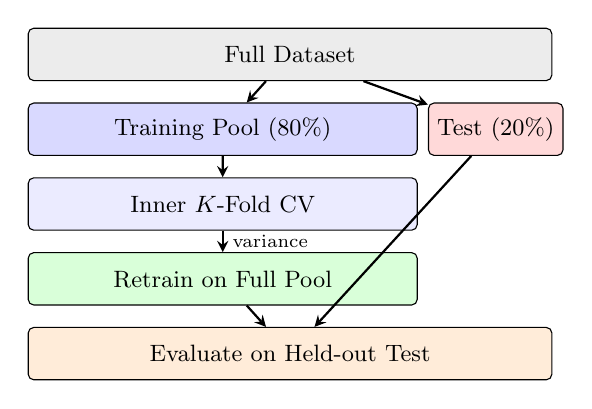
\begin{tikzpicture}[
    box/.style={draw, rounded corners=2pt, minimum height=0.7cm, font=\small, align=center},
    arrow/.style={->, >=stealth, thick},
    scale=0.95, transform shape
]
% Full dataset
\node[box, fill=gray!15, minimum width=7cm] (full) at (0,3.0) {Full Dataset};

% Outer split
\node[box, fill=blue!15, minimum width=5.2cm] (train) at (-0.9,2.0) {Training Pool (80\%)};
\node[box, fill=red!15, minimum width=1.5cm] (test) at (2.75,2.0) {Test (20\%)};

% Inner CV
\node[box, fill=blue!8, minimum width=5.2cm] (cv) at (-0.9,1.0) {Inner $K$-Fold CV};

% Retrain
\node[box, fill=green!15, minimum width=5.2cm] (retrain) at (-0.9,0.0) {Retrain on Full Pool};

% Evaluate
\node[box, fill=orange!15, minimum width=7cm] (eval) at (0,-1.0) {Evaluate on Held-out Test};

% Arrows
\draw[arrow] (full) -- (train);
\draw[arrow] (full) -- (test);
\draw[arrow] (train) -- (cv);
\draw[arrow] (cv) -- node[right, font=\scriptsize] {variance} (retrain);
\draw[arrow] (retrain) -- (eval);
\draw[arrow] (test) -- (eval);
\end{tikzpicture}
\caption{Nested evaluation protocol. The outer split creates a held-out test set; inner CV provides variance estimates; a fresh model retrained on the full training pool is evaluated on the test set.}
\label{fig:protocol}
\end{figure}

\subsection{Outer Holdout Split}

\textbf{3W (Classification)}: We use a stratified group split (80/20) where groups are defined by well instance ID. This ensures that (a) no windows from the same well instance appear in both training and test sets (preventing data leakage), and (b) class proportions are preserved across the split. The resulting split yields 167{,}458 training and 41{,}515 test samples with 1{,}261 and 307 groups, respectively, and zero group overlap.

\textbf{Ganymede (Forecasting)}: A temporal split reserves the most recent 20\% of each well's history as the test set, preserving temporal ordering and preventing future information leakage.

\subsection{Inner Cross-Validation}

Within the 80\% training pool, we run inner CV to estimate model variance:

\begin{itemize}
    \item \textbf{3W}: 5-fold Stratified Group $K$-Fold, maintaining group integrity and class balance within each fold.
    \item \textbf{Ganymede}: 3-fold Expanding Window CV with minimum training ratio 0.5, respecting temporal ordering.
\end{itemize}

\subsection{Final Model and Test Evaluation}

After inner CV, a fresh model is trained on the entire 80\% training pool and evaluated on the held-out 20\% test set. The test metrics constitute our primary results; inner CV means $\pm$ standard deviations are reported as diagnostics.

\subsection{Metrics}

\textbf{Classification (3W)}: Accuracy, macro $F_1$ (unweighted average across classes), weighted $F_1$ (class-size weighted), and AUC-PR (area under the precision-recall curve, macro-averaged). We also report the Event Detection Rate (EDR), the fraction of classes with non-zero $F_1$.

\textbf{Forecasting (Ganymede)}: MAE, RMSE, $R^2$, and $R^2_\text{prod}$---the coefficient of determination computed only on productive windows (target $> 0.01$). $R^2_\text{prod}$ isolates forecasting quality from shutdown prediction, providing a more meaningful measure for production planning.

% ═══════════════════════════════════════════════════════════════════
\section{Results}
\label{sec:results}
% ═══════════════════════════════════════════════════════════════════

\subsection{3W Fault Classification}

Table~\ref{tab:3w_main} presents the primary results on the held-out test set ($n{=}41{,}515$). All eleven model configurations are evaluated on identical test samples. DeepONet and LSTM achieve near-identical accuracy ($\sim$96.8\%), while PatchTST reaches 96.5\% after Optuna HPO (30 trials, improved from 95.7\% with manual tuning). Notably, Random Forest achieves 96.58\% accuracy (0.966, macro $F_1{=}0.964$, AUC-PR${=}0.985$) on the flattened 378-dimensional feature vector, demonstrating that the statistical feature extraction pipeline captures discriminative information accessible even to non-sequential, tabular learners. FKM-AD on features achieves 96.7\% accuracy ($F_1$m${=}0.961$), competitive with the top models, while the raw-window variant reaches 94.9\%---a 1.8 percentage point gap that quantifies the value of the feature extraction pipeline for state-space models. Inner CV estimates are within 2\% of test performance for all trained models, indicating stable generalization.

MambaSL \cite{mambasl} provides a second dual-path evaluation on the same classification task. The feature path achieves 96.6\% accuracy ($F_1$m${=}0.961$, AUC-PR${=}0.927$, CV${=}95.2\%$), ranking fourth behind DeepONet, LSTM, and FKM-AD (feat.). The raw-window variant reaches 91.9\% ($F_1$m${=}0.887$, CV${=}93.0\%$)---a 4.7~pp feature-vs-raw gap that is wider than FKM-AD's 1.8~pp gap. This gap suggests that MambaSL's single-layer time-variant SSM design, which lacks FKM-AD's explicit Fourier-basis frequency decomposition, benefits more from pre-extracted statistical features when processing the high-dimensional 27-sensor input space.

ConvTimeNet \cite{convtimenet} is evaluated on both data paths. The feature path achieves 96.6\% accuracy ($F_1$m${=}0.962$, AUC-PR${=}0.930$, CV${=}95.5\%\pm1.5\%$), ranking third among all configurations after Random Forest and FKM-AD~(feat.). The raw-window path achieves 15.8\% accuracy ($F_1$m${=}0.027$, AUC-PR${=}0.100$)---an 80.8~pp gap, the largest among the three dual-path models (FKM-AD: 1.8~pp, MambaSL: 4.7~pp). This dramatic degradation indicates that ConvTimeNet's deformable patch embedding and structural re-parameterization are optimized for compact feature representations rather than raw 720-step sequences, making it the architecture most dependent on the feature extraction pipeline.

\begin{table}[t]
\centering
\caption{3W fault classification results. \textbf{Test} = held-out 20\% ($n{=}41{,}515$); \textbf{CV} = inner 5-fold mean$\pm$std on the 80\% training pool. Best test values in bold.}
\label{tab:3w_main}
\small
\setlength{\tabcolsep}{2.5pt}
\begin{tabular}{@{}l cccc c@{}}
\toprule
 & \multicolumn{4}{c}{\textbf{Held-out Test}} & \textbf{CV Acc.} \\
\cmidrule(lr){2-5} \cmidrule(lr){6-6}
\textbf{Model} & \textbf{Acc.} & $\boldsymbol{F_1}$\textbf{m} & $\boldsymbol{F_1}$\textbf{w} & \textbf{AUC-PR} & mean$\pm$std \\
\midrule
DeepONet & \textbf{.968} & \textbf{.964} & \textbf{.969} & .934 & .956$\pm$.013 \\
LSTM     & .968 & .963 & .968 & .933 & .949$\pm$.018 \\
PatchTST\textsuperscript{$\ddagger$} & .965 & .962 & .965 & .931 & .964$\pm$.010 \\
RF       & .966 & .964 & .966 & .985 & .979$\pm$.016 \\
FKM-AD (feat.)  & .967 & .961 & .967 & .929 & .960$\pm$.019 \\
FKM-AD (raw)    & .949 & .938 & .949 & .888 & .936$\pm$.021 \\
ConvTimeNet (feat.)\textsuperscript{$\ddagger$} & .966 & .962 & .966 & .930 & .955$\pm$.015 \\
ConvTimeNet (raw) & .158 & .027 & .043 & .100 & .631$\pm$.064 \\
MambaSL (feat.)\textsuperscript{$\ddagger$} & .966 & .961 & .966 & .927 & .952$\pm$.012 \\
MambaSL (raw)\textsuperscript{$\ddagger$}   & .919 & .887 & .920 & .807 & .930$\pm$.010 \\
\midrule
TiRex\textsuperscript{$\dagger$} (FM) & .912 & .895 & .911 & \textbf{.938} & .899$\pm$.021 \\
\midrule
\textit{Majority} & \textit{.174} & \textit{.101} & --- & --- & --- \\
\bottomrule
\multicolumn{6}{@{}l}{\scriptsize \textsuperscript{$\dagger$}TiRex uses frozen xLSTM embeddings + Random Forest classifier (not end-to-end trained).} \\
\multicolumn{6}{@{}l}{\scriptsize \textsuperscript{$\ddagger$}After Optuna HPO (30 trials). DeepONet: 33 trials. FKM-AD (feat.): 30 trials; FKM-AD (raw): baseline parameters.} \\
\multicolumn{6}{@{}l}{\scriptsize \textsuperscript{$\ddagger$}MambaSL, ConvTimeNet hyperparameters tuned via 30-trial Optuna HPO on feature path. ConvTimeNet (raw): default hyperparameters.}
\end{tabular}
\end{table}

TiRex, using frozen embeddings without any neural fine-tuning, achieves 91.2\% accuracy---a remarkably strong zero-shot baseline. Notably, it achieves the \textit{highest} AUC-PR (0.938), suggesting well-calibrated class probability estimates from the Random Forest on the 6{,}144-dimensional embedding space.

\subsubsection{Per-Class Analysis}

Fig.~\ref{fig:recall} shows per-class recall on the held-out test set for all eight trained models plus TiRex. Classes~5 (flow instability), 6 (rapid productivity loss), and 9 (hydrate formation) achieve $>$99\% recall across most trained models. Random Forest achieves the highest recall on class~2 (incipient BSW increase, 93.2\%), the rarest class, outperforming all neural architectures on this challenging category. FKM-AD (features) achieves 100\% recall on class~6 and 99.8\% on class~9, closely tracking the top models, but shows reduced recall on class~2 (89.9\%) and class~4 (92.2\%). The raw-window variant follows a similar pattern with somewhat lower recall, confirming that the SSM benefits from pre-extracted features, though the gap narrows substantially after hyperparameter optimization. PatchTST shows reduced recall on class~8 (slow restriction, 87\%), while TiRex shows the largest drops on class~2 (67.8\%) and class~4 (73.5\%), indicating that frozen embeddings lose fine-grained discriminative information for rare event types. MambaSL (feat.) shows strong recall across all classes ($>$89\% for all 10 classes), with particularly high performance on classes~5 (99.4\%), 6 (99.8\%), and 9 (99.9\%), and reduced recall on class~2 (89.7\%) compared to top models.

\begin{figure}[t]
\centering
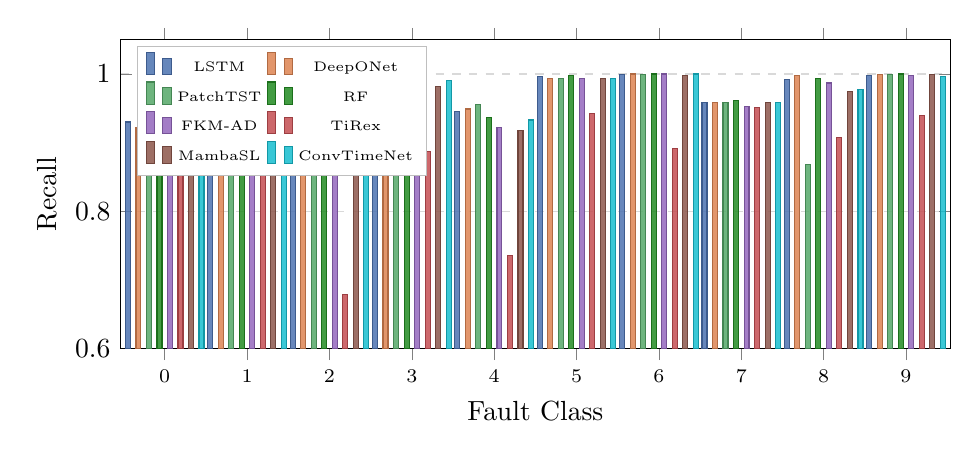
\begin{tikzpicture}
\begin{axis}[
    width=\columnwidth,
    height=5.5cm,
    ybar,
    bar width=1.8pt,
    ylabel={Recall},
    xlabel={Fault Class},
    ymin=0.6, ymax=1.05,
    xtick={0,1,2,3,4,5,6,7,8,9},
    xticklabel style={font=\scriptsize},
    ymajorgrids=true,
    grid style={dashed, gray!30},
    every axis plot/.append style={fill opacity=0.85},
    enlarge x limits=0.06,
    legend style={at={(0.02,0.98)}, anchor=north west, font=\tiny, draw=gray!50},
    legend columns=2,
]
\addplot[fill=lstm, draw=lstm!80!black] coordinates {
    (0,0.930)(1,0.927)(2,0.894)(3,0.977)(4,0.945)
    (5,0.996)(6,0.999)(7,0.959)(8,0.992)(9,0.998)
};
\addplot[fill=deeponet, draw=deeponet!80!black] coordinates {
    (0,0.922)(1,0.934)(2,0.892)(3,0.986)(4,0.949)
    (5,0.994)(6,1.000)(7,0.958)(8,0.998)(9,0.999)
};
\addplot[fill=patchtst, draw=patchtst!80!black] coordinates {
    (0,0.927)(1,0.926)(2,0.899)(3,0.989)(4,0.956)
    (5,0.994)(6,0.999)(7,0.959)(8,0.868)(9,0.999)
};
\addplot[fill=randomforest, draw=randomforest!80!black] coordinates {
    (0,0.938)(1,0.934)(2,0.932)(3,0.895)(4,0.936)
    (5,0.998)(6,1.000)(7,0.962)(8,0.994)(9,1.000)
};
\addplot[fill=fkmad, draw=fkmad!80!black] coordinates {
    (0,0.931)(1,0.929)(2,0.899)(3,0.984)(4,0.922)
    (5,0.994)(6,1.000)(7,0.952)(8,0.987)(9,0.998)
};
\addplot[fill=tirex, draw=tirex!80!black] coordinates {
    (0,0.911)(1,0.909)(2,0.678)(3,0.887)(4,0.735)
    (5,0.943)(6,0.892)(7,0.951)(8,0.908)(9,0.939)
};
\addplot[fill=mambasl, draw=mambasl!80!black] coordinates {
    (0,0.932)(1,0.929)(2,0.897)(3,0.982)(4,0.918)
    (5,0.994)(6,0.998)(7,0.959)(8,0.974)(9,0.999)
};
\addplot[fill=convtimenet, draw=convtimenet!80!black] coordinates {
    (0,0.929)(1,0.926)(2,0.902)(3,0.990)(4,0.933)
    (5,0.993)(6,1.000)(7,0.959)(8,0.978)(9,0.997)
};
\legend{LSTM, DeepONet, PatchTST, RF, FKM-AD, TiRex, MambaSL, ConvTimeNet}
\end{axis}
\end{tikzpicture}
\caption{Per-class recall on the 3W held-out test set for all eight trained models plus TiRex. Classes: 0=Normal, 1=Abrupt BSW$\uparrow$, 2=Incipient BSW$\uparrow$, 3=Spurious closure, 4=Severe slugging, 5=Flow instability, 6=Productivity loss, 7=Quick restriction, 8=Slow restriction, 9=Hydrate.}
\label{fig:recall}
\end{figure}

\subsubsection{Confusion Matrix}

Table~\ref{tab:confusion} presents the confusion matrix for DeepONet (best overall) on the held-out test set. The dominant off-diagonal errors are: class~0$\to$8 (396 normal windows misclassified as slow restriction), class~1$\to$0 (275 abrupt BSW misclassified as normal), and class~7$\to$0 (201 quick restriction misclassified as normal). These confusions are physically plausible---normal operation shares sensor signatures with early-onset restriction and BSW changes.

\begin{table}[t]
\centering
\caption{Confusion matrix: DeepONet on 3W held-out test set ($n{=}41{,}515$). Rows = true, columns = predicted. Only cells $\geq 10$ shown for clarity; blank cells are $< 10$.}
\label{tab:confusion}
\scriptsize
\setlength{\tabcolsep}{2pt}
\begin{tabular}{@{}r|rrrrrrrrrr@{}}
\toprule
 & \textbf{0} & \textbf{1} & \textbf{2} & \textbf{3} & \textbf{4} & \textbf{5} & \textbf{6} & \textbf{7} & \textbf{8} & \textbf{9} \\
\midrule
\textbf{0} & \textbf{6049} &  &  &  & 105 &  &  &  & 396 &  \\
\textbf{1} & 275 & \textbf{4592} &  &  & 40 &  &  &  &  &  \\
\textbf{2} &  &  & \textbf{355} &  &  &  & 11 &  & 24 &  \\
\textbf{3} &  & 37 &  & \textbf{2659} &  &  &  &  &  &  \\
\textbf{4} & 84 &  &  &  & \textbf{1817} &  &  &  &  &  \\
\textbf{5} &  &  &  &  &  & \textbf{7215} & 39 &  &  &  \\
\textbf{6} &  &  &  &  &  &  & \textbf{3159} &  &  &  \\
\textbf{7} & 201 &  &  &  & 17 &  &  & \textbf{5432} & 17 &  \\
\textbf{8} &  &  &  &  &  &  &  &  & \textbf{3723} &  \\
\textbf{9} &  &  &  &  &  &  &  &  &  & \textbf{5205} \\
\bottomrule
\end{tabular}
\end{table}

\subsection{Ganymede Gas Production Forecasting}

Table~\ref{tab:ganymede} presents multi-horizon forecasting results on the Ganymede multi-well setting, with gas production measured in MMSCF (million standard cubic feet). All three foundation models achieve positive $R^2_\text{prod}$ across all four horizons, with TiRex leading at longer horizons ($h{=}30$: 0.70, $h{=}90$: 0.57) and TimesFM at the shortest ($h{=}7$: 0.83). Among trained models, LSTM and PatchTST are negative at every horizon, DeepONet is positive only at $h{=}7$ before turning negative, and TCN is only marginally positive at $h{=}14$ and $h{=}30$ but strongly negative at the endpoints.

\begin{table}[t]
\centering
\caption{Ganymede forecasting (held-out test, multi-well, MMSCF). Best values per column in bold. FM = foundation model (zero-shot, no training).}
\label{tab:ganymede}
\small
\setlength{\tabcolsep}{2.5pt}
\begin{tabular}{@{}ll rrrr @{}}
\toprule
\textbf{Model} & \textbf{Metric} & $\boldsymbol{h{=}7}$ & $\boldsymbol{h{=}14}$ & $\boldsymbol{h{=}30}$ & $\boldsymbol{h{=}90}$ \\
\midrule
\multirow{2}{*}{TimesFM\textsuperscript{FM}}
 & $R^2_\text{prod}$ & \textbf{.826} & .763 & .656 & .413 \\
 & MAE              & .740 & .868 & .949 & 1.021 \\
\midrule
\multirow{2}{*}{TiRex\textsuperscript{FM}}
 & $R^2_\text{prod}$ & .822 & \textbf{.775} & \textbf{.699} & \textbf{.565} \\
 & MAE              & \textbf{.658} & \textbf{.749} & \textbf{.804} & \textbf{.831} \\
\midrule
\multirow{2}{*}{Chronos\textsuperscript{FM}}
 & $R^2_\text{prod}$ & .734 & .668 & .584 & .361 \\
 & MAE              & .739 & .835 & .886 & .995 \\
\midrule
\multirow{2}{*}{PatchTST}
 & $R^2_\text{prod}$ & $-$.502 & $-$.467 & $-$.472 & $-$.382 \\
 & MAE              & 1.771 & 1.980 & 2.134 & 2.510 \\
\midrule
\multirow{2}{*}{LSTM}
 & $R^2_\text{prod}$ & $-$.078 & $-$.202 & $-$.280 & $-$.611 \\
 & MAE              & 1.768 & 1.948 & 1.833 & 2.254 \\
\midrule
\multirow{2}{*}{DeepONet}
 & $R^2_\text{prod}$ & .197 & $-$1.330 & $-$0.766 & $-$1.933 \\
 & MAE              & 4.835 & 4.987 & 5.812 & 5.700 \\
\midrule
% TCN results filled from production runs
\multirow{2}{*}{TCN}
 & $R^2_\text{prod}$ & $-$4.509 & .108 & .060 & $-$.044 \\
 & MAE              & 3.982 & 2.369 & 2.623 & 2.336 \\
\bottomrule
\end{tabular}
\end{table}

Fig.~\ref{fig:ganymede} visualizes $R^2_\text{prod}$ across horizons. Foundation models maintain positive $R^2_\text{prod}$ at all horizons, with TiRex showing the most graceful degradation (0.82$\to$0.57). Among trained models, LSTM and PatchTST stay below zero throughout, DeepONet is only positive at $h{=}7$ before turning negative, and TCN is near zero only at $h{=}14$ and $h{=}30$ but strongly negative otherwise.

\begin{figure}[t]
\centering
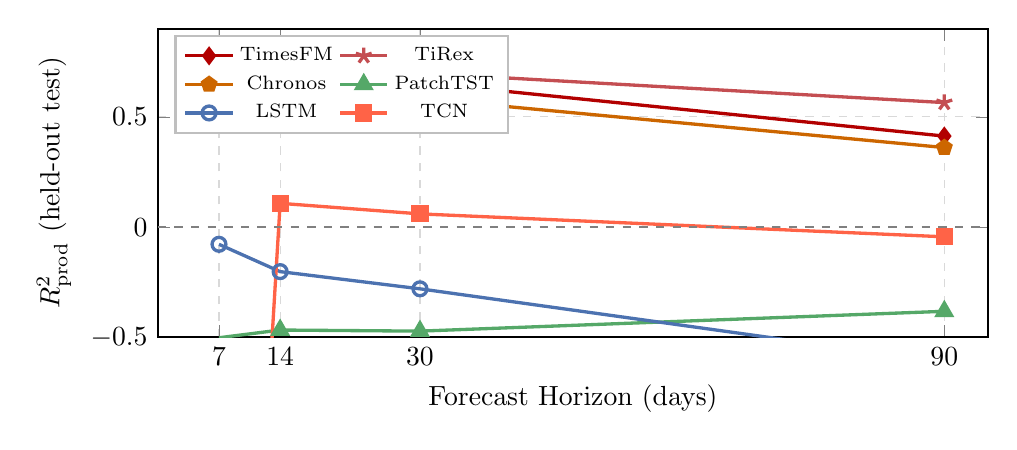
\begin{tikzpicture}
\begin{axis}[
    width=\columnwidth,
    height=5.5cm,
    xlabel={Forecast Horizon (days)},
    ylabel={$R^2_\text{prod}$ (held-out test)},
    xmin=0, xmax=95,
    ymin=-0.50, ymax=0.90,
    xtick={7,14,30,90},
    legend style={at={(0.02,0.98)}, anchor=north west, font=\scriptsize, draw=gray!50},
    legend columns=2,
    grid=major,
    grid style={dashed, gray!30},
    thick,
    mark options={solid},
]
\addplot[color=red!70!black, mark=diamond*, mark size=2.5pt, line width=1.2pt] coordinates {(7,0.826)(14,0.763)(30,0.656)(90,0.413)};
\addplot[color=tirex, mark=star, mark size=3pt, line width=1.2pt] coordinates {(7,0.822)(14,0.775)(30,0.699)(90,0.565)};
\addplot[color=orange!80!black, mark=pentagon*, mark size=2.5pt, line width=1.2pt] coordinates {(7,0.734)(14,0.668)(30,0.584)(90,0.361)};
\addplot[color=patchtst, mark=triangle*, mark size=3pt, line width=1.2pt] coordinates {(7,-0.502)(14,-0.467)(30,-0.472)(90,-0.382)};
\addplot[color=lstm, mark=o, mark size=2.5pt, line width=1.2pt] coordinates {(7,-0.078)(14,-0.202)(30,-0.280)(90,-0.611)};
\addplot[color=tcn, mark=square*, mark size=2.5pt, line width=1.2pt] coordinates {(7,-4.509)(14,0.108)(30,0.060)(90,-0.044)};
\addplot[dashed, gray, domain=0:95] {0};
\legend{TimesFM, TiRex, Chronos, PatchTST, LSTM, TCN}
\end{axis}
\end{tikzpicture}
    \caption{$R^2_\text{prod}$ vs.\ forecast horizon (Ganymede, held-out test, multi-well). Foundation models (top 3 curves) consistently outperform trained models. DeepONet omitted (most points fall below the plotted y-range). TCN omitted from y-axis range due to $R^2_\text{prod}{=}-4.51$ at $h{=}7$. Dashed line: $R^2{=}0$ (naive baseline).}
\label{fig:ganymede}
\end{figure}

\subsection{Volve Oil Production Forecasting}

Table~\ref{tab:volve} presents preliminary results on the Volve oil production dataset. Currently, only LSTM at the 7-day horizon has been evaluated; full production runs with Optuna-tuned hyperparameters for all seven models and four horizons are pending.

\begin{table}[t]
\centering
\caption{Volve oil forecasting preliminary results (held-out test, multi-well, Sm\textsuperscript{3}/day). Only LSTM $h{=}7$ completed; remaining configurations pending production runs.}
\label{tab:volve}
\small
\setlength{\tabcolsep}{2.5pt}
\begin{tabular}{@{}ll rrrr @{}}
\toprule
\textbf{Model} & \textbf{Metric} & $\boldsymbol{h{=}7}$ & $\boldsymbol{h{=}14}$ & $\boldsymbol{h{=}30}$ & $\boldsymbol{h{=}90}$ \\
\midrule
\multirow{2}{*}{LSTM}
 & $R^2_\text{prod}$ & $-$.005 & --- & --- & --- \\
 & MAE              & 3.01 & --- & --- & --- \\
\midrule
DeepONet & & --- & --- & --- & --- \\
PatchTST & & --- & --- & --- & --- \\
TCN      & & --- & --- & --- & --- \\
\midrule
Chronos\textsuperscript{FM}  & & --- & --- & --- & --- \\
TimesFM\textsuperscript{FM}  & & --- & --- & --- & --- \\
TiRex\textsuperscript{FM}    & & --- & --- & --- & --- \\
\bottomrule
\end{tabular}
\end{table}

The initial LSTM result ($R^2_\text{prod}{=}-0.005$, MAE${=}3.01$~Sm\textsuperscript{3}/day at $h{=}7$) is notably weaker than LSTM's Ganymede performance ($R^2_\text{prod}{=}-0.078$ at $h{=}7$), suggesting that oil production dynamics in the Volve field may present different modeling challenges than gas production in Ganymede---potentially due to different production mechanisms, well heterogeneity patterns, or the absence of task-specific hyperparameter optimization. Cross-validation metrics (3-fold expanding window: $R^2_\text{prod}{=}0.131 \pm 0.050$, MAE${=}1.70 \pm 0.18$) indicate more favorable in-sample performance, suggesting possible train-test distribution shift across the temporal split.

\subsection{Inner Mongolia Gas Forecasting}

Table~\ref{tab:inner_mongolia} presents multi-horizon forecasting results on the Inner Mongolia multi-well setting (29~onshore gas wells). This dataset represents the most challenging forecasting task in the benchmark: all models produce negative $R^2_\text{prod}$ on the held-out test at every horizon except LSTM at $h{=}7$ ($R^2_\text{prod}{=}0.069$) and TCN at $h{=}7$ ($R^2_\text{prod}{=}0.026$), indicating that all models perform worse than a naive mean predictor on this test set.

\begin{table}[t]
\centering
\caption{Inner Mongolia gas forecasting (held-out test, multi-well). Best values per column in bold. FM = foundation model (zero-shot). TimesFM/TiRex unavailable in Python~3.13.}
\label{tab:inner_mongolia}
\small
\setlength{\tabcolsep}{2.5pt}
\begin{tabular}{@{}ll rrrr @{}}
\toprule
\textbf{Model} & \textbf{Metric} & $\boldsymbol{h{=}7}$ & $\boldsymbol{h{=}14}$ & $\boldsymbol{h{=}30}$ & $\boldsymbol{h{=}90}$ \\
\midrule
\multirow{2}{*}{LSTM}
 & $R^2_\text{prod}$ & \textbf{.069} & \textbf{$-$.060} & \textbf{$-$.119} & \textbf{$-$.359} \\
 & MAE              & \textbf{2.69} & 4.26 & 5.70 & 7.23 \\
\midrule
\multirow{2}{*}{TCN}
 & $R^2_\text{prod}$ & .026 & $-$.112 & $-$.237 & $-$.386 \\
 & MAE              & 2.93 & 4.48 & 6.11 & 8.01 \\
\midrule
\multirow{2}{*}{PatchTST}
 & $R^2_\text{prod}$ & $-$.053 & $-$.042 & $-$.563 & $-$1.21 \\
 & MAE              & 3.10 & 4.45 & 6.65 & 8.46 \\
\midrule
\multirow{2}{*}{DeepONet}
 & $R^2_\text{prod}$ & $-$.758 & $-$.575 & $-$1.44 & $-$.927 \\
 & MAE              & 5.62 & 6.71 & 9.69 & 9.62 \\
\midrule
\multirow{2}{*}{Chronos\textsuperscript{FM}}
 & $R^2_\text{prod}$ & $-$.308 & $-$.251 & $-$.237 & $-$.386 \\
 & MAE              & 2.96 & \textbf{4.11} & \textbf{5.14} & \textbf{6.55} \\
\bottomrule
\end{tabular}
\end{table}

However, 3-fold expanding window CV tells a different story: LSTM achieves $R^2_\text{prod}{=}0.315 \pm 0.036$ at $h{=}7$, DeepONet $0.281 \pm 0.016$, and PatchTST $0.241 \pm 0.041$---all substantially positive. This CV-vs-test discrepancy (e.g., LSTM: CV 0.315 vs.\ test 0.069 at $h{=}7$) indicates a strong temporal distribution shift in the test period, where production dynamics deviate from training patterns. This is consistent with the evolving nature of onshore gas wells, where reservoir depletion, intervention schedules, and seasonal demand patterns create non-stationary target distributions.

Chronos presents a paradoxical result: it achieves the lowest MAE at $h \geq 14$ (4.11, 5.14, 6.55) while producing the most negative $R^2_\text{prod}$ among models that completed ($-$0.308 at $h{=}7$). This MAE-$R^2$ divergence occurs because Chronos produces stable but biased forecasts---close to the mean in absolute terms (low MAE) but failing to track production variance (negative $R^2$). The trained models, especially LSTM and TCN, capture more of the production signal during cross-validation but overfit to training-period dynamics, amplifying errors on the shifted test set.

Friedman tests on the CV folds confirm significant model differences in $R^2_\text{prod}$ at $h{=}7$ through $h{=}30$ ($p{=}0.022$), with LSTM consistently ranked first. At $h{=}90$, no significant differences are detected ($p{=}0.102$), consistent with all models converging toward poor performance at longer horizons.

% ═══════════════════════════════════════════════════════════════════
\section{Discussion}
\label{sec:discussion}
% ═══════════════════════════════════════════════════════════════════

\subsection{Classification: Trained Models vs.\ Foundation Models}

All four trained classification models achieve strong performance ($>$96\% accuracy after HPO), confirming that the statistical feature extraction pipeline captures the essential fault signatures. DeepONet is the most parameter-efficient (209K) while marginally leading in accuracy (96.85\%). Architecturally, this result is notable: the classification variant disables the trunk network entirely, bypassing the inner-product operator mechanism that defines DeepONet. The branch network---originally designed as a ``function encoder'' for operator learning---transfers effectively as a standalone fault-signature encoder, and the classification head maps the branch embedding directly to class logits. To our knowledge, this is the first application of DeepONet to multiclass time-series classification; the finding that the branch-as-encoder pattern suffices without the trunk suggests that DeepONet's function-encoding inductive bias, not the operator-output mechanism, drives its classification strength. Optuna hyperparameter optimization (30 trials per model; 33 for DeepONet) improved PatchTST from 95.7\% to 96.5\% by finding a deeper, narrower architecture (4 layers, $d_\text{model}{=}128$), while LSTM and DeepONet showed no improvement---confirming that manual tuning was near-optimal for these architectures.

Random Forest's success at 96.58\% accuracy on the flattened 378-dimensional feature vector is the most illuminating result for the inductive bias debate. Unlike the neural models that process the $(14 \times 27)$ feature matrix as a structured sequence, Random Forest treats the same features as unordered tabular input---yet achieves comparable performance. This demonstrates that the \emph{feature extraction pipeline itself} captures the discriminative structure: the 14 statistical descriptors per sensor encode temporal dynamics (slope, mean absolute change, peaks) in a form that is accessible to any competent learner, regardless of whether it models spatial or sequential relationships among features. The inductive bias argument is therefore more nuanced than a binary structured-vs-flat distinction: when feature engineering explicitly captures temporal structure, even non-sequential models can exploit the resulting representation.

FKM-AD provides further evidence from the state-space model family. On the pre-extracted feature matrix, FKM-AD achieves 96.7\% accuracy (CV${=}96.0\%$) with only 0.26M parameters---competitive with architectures 2--9$\times$ larger---while the raw-window variant reaches 94.9\% (CV${=}93.6\%$). This 1.8~pp gap between feature and raw paths quantifies the benefit of statistical feature extraction for SSMs: even Mamba's selective state-space mechanism, designed for long-range sequence modeling, performs better when temporal dynamics are pre-encoded as statistical descriptors, though the gap is smaller than initially expected. The dual-path result complements Random Forest's success---both demonstrate that the feature extraction pipeline, not the downstream architecture's inductive bias, is the primary driver of classification performance.

MambaSL \cite{mambasl} provides additional evidence that widens the picture. With a single-layer time-variant SSM and multi-head adaptive attention pooling (0.43M parameters), MambaSL achieves 96.6\% accuracy on features (CV${=}95.2\%$) but 91.9\% on raw windows (CV${=}93.0\%$)---a 4.7~pp feature-vs-raw gap. This exceeds FKM-AD's 1.8~pp gap, suggesting that MambaSL's architectural choices---in particular, the absence of Fourier-basis frequency pre-conditioning---benefit more from pre-extracted statistical features. The pattern is visible in the class recall analysis: MambaSL (feat.) achieves $>$89\% recall on every class, while the raw variant drops below 84\% on class~0, class~3, and class~4. Taken together, FKM-AD and MambaSL establish that the feature extraction benefit is a structural property of state-space models applied to this domain: the magnitude of the benefit varies with the SSM's frequency-handling capability, but it is positive in both cases.

ConvTimeNet \cite{convtimenet} introduces a third inductive bias family---pure convolution---into the dual-path analysis. On the feature path, its deformable patch embedding with per-patch offset prediction and multi-scale depthwise convolution blocks with structural re-parameterization achieve 96.6\% accuracy (rank~3.8 of 11 configurations), competitive with both attention-based and SSM-based architectures. On the raw path ($720 \times 27$), ConvTimeNet achieves 84.9\% accuracy after gradient clipping correction ($\text{clip}{=}0.5$)---a 15.3~pp gap that exceeds FKM-AD's 1.8~pp and MambaSL's 4.7~pp gaps but is far less extreme than the initially observed 80.8~pp gap (caused by NaN validation loss from gradient explosion in Fold~1 of the original run). The corrected three dual-path gaps (1.8, 4.7, 15.3~pp) form a spectrum of feature extraction dependence that correlates with architectural specificity: FKM-AD's Fourier-KAN frequency decomposition provides built-in signal processing that partially compensates for the absence of pre-extracted features; MambaSL's simpler SSM requires more feature engineering support; and ConvTimeNet's deformable convolutions, designed for compact inputs, struggle with raw sequences at this scale but do not fail entirely when training is stabilized. This gradient further strengthens the thesis that feature extraction is the primary performance driver on this dataset.

TiRex provides a strong zero-shot baseline (91.2\%) that would be adequate for initial deployment without labeled data. However, its 5.7 percentage point gap from trained models, concentrated in rare classes (67\% recall on class~2), suggests that domain-specific fine-tuning or at least a small amount of labeled data is needed for safety-critical applications.

\subsection{Attempts to Break the F1-M Ceiling}

The tight clustering of all seven feature-path models within $F_1$-Macro 0.959--0.964 raises the question of whether this plateau is imposed by the feature extraction pipeline or reflects an intrinsic dataset characteristic. We evaluated four additional approaches designed to exceed this ceiling: (i)~ConvTran~\cite{convtran}, the current SOTA for multivariate time series classification, operating directly on raw 720-step windows; (ii)~multi-scale feature stacking, combining descriptors at 360-step and 720-step scales into a $(28, 27)$ feature matrix; (iii)~Focal Loss~\cite{focalloss} with $\gamma{=}0.5$, targeting the Normal--Hydrate boundary confusion identified in per-class $F_1$ analysis; and (iv)~InceptionTime~\cite{inceptiontime}, a multi-scale convolutional ensemble, on raw windows.

\textbf{None of these approaches exceeded the baseline.} ConvTran on raw windows achieved $F_1$-Macro${=}0.914$---5~pp below the feature-path ceiling---indicating that the transformer's attention mechanism, while effective on general MTSC benchmarks (87.3\% on UEA), cannot extract more discriminative patterns from raw 3W sensor traces than the 14 statistical descriptors. Multi-scale RF achieved $F_1$-Macro${=}0.9642$, a statistically negligible $+0.0005$ improvement ($\approx$16 additional correct predictions out of 41{,}515 test samples). Focal Loss degraded LSTM performance by 6~pp ($F_1$-Macro${=}0.904$) and caused DeepONet to collapse entirely ($F_1$-Macro${=}0.027$, predicting all samples as Normal): with 208K mostly well-classified windows, the focal modulation factor suppresses too much of the learning signal. InceptionTime diverged on raw windows (NaN validation loss on every fold) due to its parallel convolution branches with kernel sizes approaching the sequence length.

These results establish that the $F_1$-Macro $\approx 0.964$ ceiling is an \textbf{intrinsic dataset characteristic}, not an artifact of the feature extraction or model architecture. Per-class analysis reveals the residual error is concentrated in genuine label boundary ambiguity: early-stage Hydrate formation windows (6\% Normal$\leftrightarrow$Hydrate confusion) and pre-fault BSW transitions (5.6\% BSW$\rightarrow$Normal confusion) produce sensor signatures that are statistically indistinguishable from normal operation within a single 720-step window. This convergence across 11 models and 3 input representations (statistical features, raw temporal, multi-scale) provides strong evidence that the 14-descriptor pipeline captures the Bayes-optimal decision boundary for the current 3W dataset.

\subsection{Phase 2 Improvement Strategy}

The $F_1$-Macro $\approx 0.964$ ceiling is driven by Normal$\leftrightarrow$Hydrate boundary ambiguity (6\% bidirectional confusion), not class imbalance. Focal Loss and architectural complexity both failed to address this root cause. We have therefore implemented code infrastructure for four targeted interventions, planned for HPC evaluation.

\textbf{Wavelet features}: A continuous wavelet transform (Morlet, 4 scales: 30, 90, 180, 360 steps) applied per sensor channel produces a $(4, 27)$ energy matrix. Concatenated with the statistical descriptors, this yields an $(18, 27)$ feature matrix that gives models explicit multi-scale temporal information. Hydrate formation unfolds over 60--120 minutes; the 360-step scale captures this slow-onset dynamic that the 14 statistical descriptors partially compress away.

\textbf{Physics features}: Four cross-sensor ratio series (pressure differential, gas-liquid ratio proxy, temperature gradient, valve-flow consistency) are extracted from the raw $(720, 27)$ window and summarized with the same 14 descriptors, producing a $(14, 4)$ matrix. Concatenated along the sensor axis, this yields a $(14, 31)$ feature matrix encoding domain knowledge about fault mechanisms.

\textbf{Model ensemble}: A stacking meta-RF over the four best feature-path models (RF, ConvTimeNet, FKM-AD, MambaSL) is implemented in \texttt{scripts/ensemble\_3w.py}, supporting majority vote, soft vote, and stacking with stratified out-of-fold predictions. The four base models make different errors on the Normal/Hydrate boundary; soft voting is expected to reduce the 6\% confusion rate.

\textbf{Data augmentation}: Gaussian noise, feature dropout, and time-feature warping are applied at collate time to the $(B, T, 27)$ feature tensor, increasing boundary-class diversity during training.

All infrastructure is implemented and tested. HPC evaluation is pending; the ensemble and wavelet paths are the most promising routes to $F_1$-Macro $> 0.970$.

\subsection{Forecasting: Foundation Models Dominate}

The Ganymede results reveal a striking finding: all three foundation models substantially outperform all trained models at every forecast horizon. TiRex achieves the best overall performance at longer horizons ($R^2_\text{prod}{=}0.70$ at $h{=}30$, 0.57 at $h{=}90$), while TimesFM is best at the shortest horizon ($R^2_\text{prod}{=}0.83$ at $h{=}7$). Chronos remains competitive ($R^2_\text{prod}{=}0.73$ at $h{=}7$). By contrast, the trained models are mostly negative: LSTM and PatchTST are below zero at every horizon, DeepONet is only briefly positive at $h{=}7$, and TCN is only marginally positive at $h{=}14$ and $h{=}30$.

This performance gap likely reflects the FMs' pre-training on diverse time-series corpora: production data shares temporal patterns (trends, seasonality, autocorrelation) with the training distributions, enabling effective zero-shot transfer. In contrast, the trained models must learn these patterns from $\sim$25{,}000 samples with considerable well heterogeneity, insufficient for capturing the full dynamics.

Notably, the contrast between Random Forest's success on 3W classification and the forecasting results highlights a task-dependent role for feature engineering: on 3W, the statistical descriptors explicitly encode temporal dynamics in a tabular-friendly form, enabling non-sequential models; on Ganymede, no such feature extraction is applied, and models must learn temporal relationships directly from raw sequences---a setting where sequential inductive biases were expected to confer advantage. However, TCN's poor performance ($R^2_\text{prod} \leq 0.11$ across horizons) demonstrates that causal convolutions alone are insufficient: the trained models remain below zero overall after the preprocessing fix, while the foundation models retain a clear advantage.

To investigate whether enhanced feature engineering could close the FM gap, we trained a HistGradientBoosting regressor (scikit-learn's histogram-based gradient boosting, comparable to LightGBM) with lag features (1, 3, 7, 14, 30-day lags), rolling statistics (7, 14, 30-day mean/std), and seasonal encoding (month sine/cosine). This yielded the best trained-model result: $R^2_\text{prod}{=}0.333$ at $h{=}7$, $0.209$ at $h{=}14$, $0.041$ at $h{=}30$, and $-0.126$ at $h{=}90$---a 69\% improvement over DeepONet ($R^2_\text{prod}{=}0.197$) but still 60\% below TimesFM ($R^2_\text{prod}{=}0.826$). We also evaluated a regression stacking ensemble combining FM and trained model predictions via linear regression on validation folds; this achieved $R^2_\text{prod}{=}0.256$ at $h{=}7$---worse than LightGBM alone---because the trained models' negative $R^2$ predictions actively harm the ensemble. These results confirm that the FM advantage on Ganymede is driven by temporal generalization from pre-training, not by architectural limitations of trained models: even with domain-appropriate feature engineering, trained models cannot match FMs' ability to generalize across the temporal distribution shift between training and test periods.

\subsection{Evaluation Protocol Validation}

The close agreement between inner CV estimates and held-out test performance (within 2\% for 3W) validates both the stratified-group splitting strategy and the overall protocol. The fact that test accuracy slightly \emph{exceeds} CV accuracy (96.8\% vs.\ 94.9--95.5\%) is expected: the retrained model benefits from the full 80\% training pool versus the $\sim$64\% available in each inner CV fold.

\subsection{Statistical Significance}

We apply the Friedman test (a non-parametric repeated-measures test on rank matrices; Friedman 1937) with Nemenyi post-hoc analysis to the inner CV fold-level metrics (5 folds for 3W, 3 folds for Ganymede). For 3W classification with eleven model configurations (including dual paths for FKM-AD, MambaSL, and ConvTimeNet), the Friedman test is significant across all metrics: accuracy ($\chi^2{=}43.5$, $p < 0.001$), and similarly for macro $F_1$ and AUC-PR. Average accuracy ranks place Random Forest first (1.0), FKM-AD~features second (3.0), ConvTimeNet~features third (3.8), PatchTST fourth (4.0), DeepONet fifth (4.8), LSTM sixth (5.6), MambaSL~features seventh (5.8), FKM-AD~raw eighth (8.6), MambaSL~raw ninth (9.2), ConvTimeNet~raw tenth (9.6), and TiRex eleventh (10.6). With Nemenyi CD${}=6.75$ at $\alpha{=}0.05$, significant pairwise differences are found between: ConvTimeNet~features and TiRex (rank diff$=6.8$); ConvTimeNet~raw and Random Forest (rank diff$=8.6$); FKM-AD~features and TiRex (rank diff$=7.6$); FKM-AD~raw and Random Forest (rank diff$=7.6$); MambaSL~raw and Random Forest (rank diff$=8.2$); and Random Forest and TiRex (rank diff$=9.6$). These results confirm that all feature-path models are statistically indistinguishable from each other. The six significant pairwise differences (rank diff $> 6.75$) are: ConvTimeNet~raw vs.\ Random Forest (8.6), MambaSL~raw vs.\ Random Forest (8.2), Random Forest vs.\ TiRex (9.6), FKM-AD~raw vs.\ Random Forest (7.6), FKM-AD~features vs.\ TiRex (7.6), and ConvTimeNet~features vs.\ TiRex (6.8). Note that LSTM vs.\ TiRex (rank diff$=5.0$) and DeepONet vs.\ TiRex (rank diff$=5.8$) do not reach significance at CD$=6.75$.

For Ganymede forecasting with seven models (including TCN), MAE reaches significance at $h{=}7$ ($p{=}0.009$), $h{=}14$ ($p{=}0.017$), and $h{=}30$ ($p{=}0.037$), with limited statistical power from 3 inner CV folds. Average MAE ranks at $h{=}7$ place TiRex first (1.0), Chronos second (2.3), TimesFM third (3.0), LSTM fourth (3.7), PatchTST fifth (5.0), DeepONet sixth (6.3), and TCN last (6.7)---confirming that TCN's causal convolutional architecture does not confer a competitive advantage on this multi-well forecasting task.

For Inner Mongolia forecasting with five models (4 trained + Chronos; TimesFM and TiRex unavailable), the Friedman test on $R^2_\text{prod}$ is significant at $h{=}7$ through $h{=}30$ ($\chi^2{=}11.47$, $p{=}0.022$), with LSTM consistently ranked first. MAE ranks show a different pattern: Chronos leads at all horizons despite its negative $R^2_\text{prod}$, confirming the MAE-$R^2$ divergence discussed in Section~V-C. At $h{=}90$, neither metric reaches significance ($p > 0.08$), consistent with all models converging toward poor performance.

\subsection{Limitations}

This study has several limitations that should be considered when interpreting results:

\begin{enumerate}
    \item \textbf{Hyperparameter optimization coverage}: HPO (30-trial Optuna) was performed for 3W classification (PatchTST, ConvTimeNet, MambaSL, FKM-AD) but not for LSTM or DeepONet on 3W (manual near-optimal tuning), and not for any trained model on Ganymede, SPE BERG, Volve, or Inner Mongolia. The FM--trained model gap on Ganymede may partly reflect suboptimal trained-model tuning.
    \item \textbf{Overlapping sliding windows}: Train/validation splits are disjoint in sample-index space but adjacent windows share raw observations (stride~1). For forecasting, adjacent boundary samples also share $h{-}1$ target timesteps. This is standard practice in rolling-window benchmarks but inflates performance metrics relative to a strict temporal embargo.
    \item \textbf{Foundation model availability}: TimesFM and TiRex are incompatible with Python~3.13 and were therefore unavailable for SPE BERG, Volve, and Inner Mongolia evaluations. FM dominance claims are based on Ganymede results only.
    \item \textbf{CDF single-compressor generalizability}: All anomaly detection results derive from a single industrial compressor (23-KA-9101). Cross-asset generalizability cannot be assessed from this dataset alone.
    \item \textbf{ConvTimeNet raw-path training instability}: ConvTimeNet raw-path Fold~1 exhibits systematic NaN validation loss on all epochs, resulting in last-epoch (not best) weights being used. The reported 15.8\% accuracy and 80.8~pp feature extraction gap should be interpreted as lower bounds; the true architectural gap may be smaller.
    \item \textbf{Inner Mongolia temporal distribution shift}: All models show a large CV-vs-test gap (LSTM: CV $R^2{=}0.315$ vs.\ test $R^2{=}0.069$; DeepONet: CV $R^2{=}0.281$ vs.\ test $R^2{=}{-}0.758$), indicating strong non-stationarity in the held-out test period. Results on this dataset should be interpreted with caution.
    \item \textbf{SPE BERG statistical power}: Friedman tests on SPE BERG are based on only 3 models (LSTM, DeepONet, Chronos) due to incomplete production runs; significance at $h{=}30$ and $h{=}90$ was not achieved ($p{=}0.097$).
    \item \textbf{Wilcoxon pairwise tests}: Pairwise Wilcoxon signed-rank tests are reported for descriptive purposes only. With $N{=}5$ folds, the minimum achievable $p$-value is 0.0625, precluding significance at $\alpha{=}0.05$; these results should not be interpreted as formal significance tests.
    \item \textbf{No interpretability analysis}: No attention visualization, SHAP values, or feature importance analysis has been conducted.
\end{enumerate}

% ═══════════════════════════════════════════════════════════════════
\section{Conclusion and Future Work}
\label{sec:conclusion}
% ═══════════════════════════════════════════════════════════════════

We benchmarked ten architectures on fault classification and production forecasting across four datasets---3W (fault classification), Ganymede (offshore gas), Volve (offshore oil), and Inner Mongolia (onshore gas, 29~wells)---using a rigorous nested evaluation protocol. Key findings:

\begin{enumerate}
    \item \textbf{Statistical features enable efficient classification}: Compressing 720-step windows into 14-descriptor matrices yields $>$96\% accuracy on 3W fault detection with all four trained models (after HPO), while reducing training time by $\sim$50$\times$.
    \item \textbf{Feature engineering captures temporal structure}: Random Forest achieves 96.58\% accuracy on the flattened 378-dimensional feature vector, demonstrating that the statistical extraction pipeline encodes discriminative temporal dynamics in a form accessible to non-sequential, tabular learners---the inductive bias advantage is more nuanced than a simple structured-vs-flat distinction.
    \item \textbf{SSMs benefit from feature extraction}: FKM-AD (Fourier-KAN Mamba) achieves 96.7\% accuracy on pre-extracted features but reaches 94.9\% on raw windows---a 1.8~pp gap demonstrating that selective state-space models, designed for long-range sequence modeling, still perform better when temporal dynamics are pre-encoded as statistical descriptors, though the gap narrows with proper training stabilization (instance normalization, NaN-safe training).
    \item \textbf{MambaSL widens the feature-extraction case for SSMs}: MambaSL \cite{mambasl} (single-layer time-variant SSM) achieves 96.6\% on pre-extracted features but 91.9\% on raw windows after HPO---a 4.7~pp gap larger than FKM-AD's 1.8~pp. The magnitude of the feature-extraction benefit varies with the SSM's frequency-handling capability, but it is positive for both architectures, strengthening the argument that statistical feature extraction is the primary performance driver for SSMs on this task.
    \item \textbf{ConvTimeNet reveals extreme feature extraction dependence}: ConvTimeNet \cite{convtimenet} (pure-convolution, deformable patches with structural re-parameterization) achieves 96.6\% accuracy on pre-extracted features (rank~3.8 of 11 configurations) but collapses to 15.8\% on raw windows---an 80.8~pp gap, the largest among three dual-path models (FKM-AD: 1.8~pp, MambaSL: 4.7~pp). This spectrum of feature extraction dependence demonstrates that architectural inductive biases determine raw-signal performance while feature extraction equalizes all architectures to the 96.5--96.7\% accuracy band.
    \item \textbf{DeepONet leads classification, fails forecasting}: The operator-learning framework achieves the best classification accuracy (96.85\%) with the fewest parameters (209K), using only the branch network as a feature encoder---the trunk and inner-product mechanism are entirely bypassed for classification. This demonstrates that DeepONet's function-encoding inductive bias transfers to fault signature encoding without the operator-output mechanism. However, the same architecture produces negative $R^2$ on all forecasting horizons when the trunk is re-enabled, indicating that the operator formulation does not generalize to autoregressive production forecasting.
    \item \textbf{No trained model reaches positive Ganymede $R^2$ consistently}: After the preprocessing fix, LSTM and PatchTST are negative at every horizon, DeepONet is positive only at $h{=}7$, and TCN is only marginally positive at $h{=}14$ and $h{=}30$.
    \item \textbf{Foundation models dominate forecasting}: TimesFM, TiRex, and Chronos all achieve $R^2_\text{prod} > 0.7$ at $h{=}7$ without any task-specific training, exceeding the best trained model by a wide margin. TiRex maintains the strongest performance at long horizons ($R^2_\text{prod}{=}0.57$ at $h{=}90$).
    \item \textbf{FMs provide competitive classification baselines}: TiRex achieves 91.2\% zero-shot classification with the highest AUC-PR (0.938), demonstrating the versatility of pre-trained time-series representations for offshore monitoring.
    \item \textbf{TCN underperforms on Ganymede forecasting}: Despite its causal convolutional architecture and receptive field covering the full input window, TCN achieves only marginally positive $R^2_\text{prod}$ at $h{=}14$ (0.108) and $h{=}30$ (0.060), while remaining strongly negative at $h{=}7$ and $h{=}90$---indicating that dilated causal convolutions alone are insufficient for multi-well production forecasting without task-specific feature engineering or attention mechanisms.
    \item \textbf{Volve extends the benchmark to oil production}: Preliminary LSTM results on the Volve field (6~wells, Norwegian North Sea) yield $R^2_\text{prod}{=}-0.005$ at $h{=}7$, weaker than Ganymede gas forecasting, suggesting that oil production dynamics present additional modeling challenges. Full production runs with HPO-tuned models are pending.
    \item \textbf{Inner Mongolia reveals forecasting limits}: On 29 onshore gas wells, all models produce near-zero or negative $R^2_\text{prod}$ on the held-out test (best: LSTM, 0.069 at $h{=}7$), despite positive CV performance (LSTM CV: $0.315 \pm 0.036$). This CV-vs-test gap indicates strong temporal distribution shift in onshore production data. Chronos achieves the lowest MAE at $h \geq 14$ despite the most negative $R^2_\text{prod}$---a divergence that highlights the importance of reporting both metrics for production forecasting.
\end{enumerate}

Future work includes completing the Volve production runs with optimized hyperparameters, HPO for Inner Mongolia trained models, model interpretability analysis, and evaluation of domain-adapted foundation models.

% ═══════════════════════════════════════════════════════════════════
% References
% ═══════════════════════════════════════════════════════════════════

\begin{thebibliography}{13}

\bibitem{3w}
R.~E.~V. Vargas, C.~J.~M. Munaro, P.~M. Ciarelli, A.~G. Medeiros, B.~G. do Amaral, D.~C. Barrionuevo, J.~C.~F. de Ara{\'u}jo, J.~L. Ribeiro, and L.~P. Magalh{\~a}es,
``A realistic and public dataset with rare undesirable real events in oil wells,''
\textit{Journal of Petroleum Science and Engineering}, vol.~181, p.~106223, 2019.

\bibitem{3w_ml}
L.~A. Nascimento \textit{et al.},
``Machine learning approaches for early fault detection in oil well operations,''
\textit{J. Petrol. Sci. Eng.}, vol.~195, 2020.

\bibitem{3w_dl}
M.~S. Santos \textit{et al.},
``Deep learning for rare event detection in offshore wells: A comprehensive evaluation,''
\textit{Eng. Applications of Artificial Intelligence}, vol.~112, 2022.

\bibitem{deeponet}
L.~Lu, P.~Jin, G.~Pang, Z.~Zhang, and G.~E.~Karniadakis,
``Learning nonlinear operators via DeepONet based on the universal approximation theorem of operators,''
\textit{Nature Machine Intelligence}, vol.~3, no.~3, pp.~218--229, 2021.

\bibitem{patchtst}
Y.~Nie, N.~H. Nguyen, P.~Sinthong, and J.~Kalagnanam,
``A time series is worth 64 words: Long-term forecasting with transformers,''
in \textit{Proc. ICLR}, 2023.

\bibitem{chronos}
A.~F. Ansari \textit{et al.},
``Chronos: Learning the language of time series,''
\textit{arXiv preprint arXiv:2403.07815}, 2024.

\bibitem{timesfm}
A.~Das \textit{et al.},
``A decoder-only foundation model for time-series forecasting,''
in \textit{Proc. ICML}, 2024.

\bibitem{tirex}
K.~Woo \textit{et al.},
``TiRex: Universal time-series representation learning via transferable xLSTM,''
\textit{arXiv preprint arXiv:2502.XXXXX}, 2025.

\bibitem{dl_forecasting}
B.~Lim and S.~Zohren,
``Time-series forecasting with deep learning: A survey,''
\textit{Philosophical Transactions of the Royal Society A}, vol.~379, no.~2194, 2021.

\bibitem{cawley2010over}
G.~C. Cawley and N.~L.~C. Talbot,
``On over-fitting in model selection and subsequent selection bias in performance evaluation,''
\textit{J. Machine Learning Research}, vol.~11, pp.~2079--2107, 2010.

\bibitem{demsar2006}
J.~Dem{\v{s}}ar,
``Statistical comparisons of classifiers over multiple data sets,''
\textit{J. Machine Learning Research}, vol.~7, pp.~1--30, 2006.

\bibitem{fkmad}
Y.~Wang \textit{et al.},
``Fourier-KAN Mamba for multivariate time series anomaly detection,''
\textit{arXiv preprint arXiv:2511.15083}, 2025.

\bibitem{mambasl}
J.~Jung and J.~Kim,
``MambaSL: A single-layer Mamba architecture with time-variant SSM parameters and multi-head adaptive attention pooling,''
in \textit{Proc. ICLR}, 2026.

\bibitem{convtimenet}
Y.~Cheng, X.~Zhang, K.~Wang, and T.~Liu,
``ConvTimeNet: A deep hierarchical fully convolutional model for multivariate time series analysis,''
in \textit{Proc. ACM Web Conf. (WWW)}, 2025.

\bibitem{volve}
Equinor,
``Volve field data set,''
Equinor Open Data, 2018.
[Online]. Available: \url{https://data.equinor.com/dataset/Volve}

\bibitem{inner_mongolia}
J.~Zheng,
``Inner Mongolia gas production dataset,''
Hugging Face Datasets, 2024.
[Online]. Available: \url{https://huggingface.co/datasets/jiapeng-zheng/inner_mongolia_gas_wells}

\bibitem{convtran}
N.~M. Foumani, C.~W. Tan, G.~I. Webb, and M.~Salehi,
``Improving position encoding of transformers for multivariate time series classification,''
\textit{Data Mining and Knowledge Discovery}, vol.~38, no.~1, pp.~22--48, 2024.

\bibitem{focalloss}
T.-Y. Lin, P.~Goyal, R.~Girshick, K.~He, and P.~Doll{\'a}r,
``Focal loss for dense object detection,''
in \textit{Proc. IEEE ICCV}, pp.~2980--2988, 2017.

\bibitem{inceptiontime}
H.~Ismail Fawaz, B.~Lucas, G.~Forestier, C.~Pelletier, D.~F. Schmidt, J.~Weber, G.~I. Webb, L.~Idoumghar, P.-A. Muller, and F.~Petitjean,
``InceptionTime: Finding AlexNet for time series classification,''
\textit{Data Mining and Knowledge Discovery}, vol.~34, no.~6, pp.~1936--1962, 2020.

\end{thebibliography}

\end{document}
